\chapter{细胞呼吸与发酵}\label{ch:b1:respiration-fermentation}

隔绝空气的酵母糖溶液中会冒出
二氧化碳气泡，并把糖转化为酒精；让空气进入后，
气泡变慢，酒精停止生成，酵母的生长
在同样的糖上快了十倍。巴斯德于 1861 年观察到这一现象，却无法解释；
这一解释花了一个世纪才得出，贯穿
本章的全部内容。氧气使\omterm{def:b1:cell-unit-of-life:cell}{细胞}从葡萄糖中获取的能量
是无氧时的十五倍，其做法是让糖的电子
沿一串载体传给氧气，并将质子泵过
膜，再让质子回流经过一台
合成 \omterm{def:b1:water-small-molecules:atp}{ATP} 的涡轮机。本章介绍\omterm{def:b1:respiration-fermentation:glycolysis}{糖酵解}、\omterm{def:b1:respiration-fermentation:krebs}{克雷布斯
循环}、\omterm{def:b1:respiration-fermentation:chain}{呼吸链}及其化学渗透偶联，
无氧\omterm{def:b1:respiration-fermentation:fermentation}{发酵}，以及\omterm{def:b1:lipids:triglyceride}{脂肪}和
\omterm{def:b1:proteins:peptide}{蛋白质}借同一套机制的燃烧。

\section{葡萄糖的氧化}

\begin{proposition}[总反应及其各阶段]\label{prop:b1:respiration-fermentation:overview}
\index{细胞呼吸}
葡萄糖的完全氧化
\[
\mathrm{C_6H_{12}O_6} + 6\,\mathrm{O_2} \to 6\,\mathrm{CO_2} + 6\,\mathrm{H_2O},
\qquad \Delta G^{\circ\prime} = \qty{-2870}{kJ/mol},
\]
分三个阶段进行，且电子在各阶段中都不直接
与氧气相遇。\emph{\omterm{def:b1:respiration-fermentation:glycolysis}{糖酵解}}在\omterm{def:b1:eukaryotic-cell:organelle}{细胞溶胶}中将葡萄糖
分解为两分子丙酮酸，并产生 2 个 \omterm{def:b1:water-small-molecules:atp}{ATP} 和 2 个 NADH。\emph{丙酮酸
氧化与\omterm{def:b1:respiration-fermentation:krebs}{克雷布斯循环}}在\omterm{def:b1:eukaryotic-cell:mitochondrion}{线粒体}基质中将丙酮酸氧化为
$\mathrm{CO_2}$，并将电子转移到 8 个 NADH 和
2 个 $\mathrm{FADH_2}$ 上，同时产生 2 个 GTP。\emph{氧化
磷酸化}在\omterm{def:b1:eukaryotic-cell:mitochondrion}{线粒体}内膜上进行，电子经一条泵出质子的载体链
传给氧气，
质子梯度驱动约 26 个 \omterm{def:b1:water-small-molecules:atp}{ATP} 的合成。总计
每分子葡萄糖约产生 30 个 \omterm{def:b1:water-small-molecules:atp}{ATP}，约一半的\omterm{prop:b1:water-small-molecules:gibbs}{自由能}
被捕获，其余以热的形式释放。
\end{proposition}

\begin{definition}[电子载体]\label{def:b1:respiration-fermentation:carriers}
\index{NAD}\index{FAD}
\emph{$\mathrm{NAD^+}$}（烟酰胺腺\omterm{def:b1:nucleic-acids:nucleotide}{嘌呤}二\omterm{def:b1:nucleic-acids:nucleotide}{核苷酸}）从\omterm{def:b1:enzymes:enzyme}{底物}
接受两个电子和一个质子，还原为 NADH；\emph{FAD}
接受两个电子和两个质子，还原为 $\mathrm{FADH_2}$。
二者都是脱氢酶的\omterm{def:b1:enzymes:enzyme}{辅酶}，并且都可循环利用：经分解代谢
被还原，再经\omterm{def:b1:respiration-fermentation:chain}{呼吸链}重新氧化。\omterm{def:b1:cell-unit-of-life:cell}{细胞}内仅含有
微摩尔量的它们，每小时可周转数千次。
它们的氧化还原电位，$E'_0 = \qty{-0.32}{V}$ 对应 $\mathrm{NAD^+}/\mathrm{NADH}$，
使它们远低于氧气（$\qty{+0.82}{V}$）：每一对电子
由 NADH 交给氧气时释放 $\Delta G^{\circ\prime} = -2F\Delta E =
\qty{-220}{kJ/mol}$，足以合成四个以上的 \omterm{def:b1:water-small-molecules:atp}{ATP}。
\end{definition}

\begin{omfigure}
\begin{tikzpicture}[font=\footnotesize, >=Stealth, line cap=round,
  st/.style={draw, thick, rounded corners=4pt, minimum height=9mm, text width=30mm, align=center, fill=white}]
  \node[st, fill=omDef!12] (gly) at (0,0) {\textbf{糖酵解}\\ 细胞溶胶 \\ 葡萄糖 $\to$ 2 丙酮酸};
  \node[st, fill=omProp!12] (krebs) at (5.4,0) {\textbf{丙酮酸氧化}\\ \textbf{+ 克雷布斯循环}\\ 基质；2 丙酮酸 $\to$ 6 $\mathrm{CO_2}$};
  \node[st, fill=omThm!12] (ox) at (10.8,0) {\textbf{氧化磷酸化}\\ 线粒体内膜；$\mathrm{O_2} \to \mathrm{H_2O}$};
  \draw[->, very thick] (gly) -- (krebs) node[midway, above, font=\scriptsize] {2 丙酮酸};
  \draw[->, very thick] (krebs) -- (ox) node[midway, above, align=center, font=\scriptsize] {8 NADH\\ 2 $\mathrm{FADH_2}$};
  \draw[->, very thick] (gly.north) .. controls (0,1.8) and (10.8,1.8) .. (ox.north) node[pos=0.5, above] {2 NADH};
  \node[anchor=north, omExo!70!black] at (gly.south) {2 ATP};
  \node[anchor=north, omExo!70!black] at (krebs.south) {2 GTP};
  \node[anchor=north, omExo!70!black] at (ox.south) {$\approx$ 26 ATP};
  \node[anchor=north, align=center, gray] at (5.4,-1.75) {每分子葡萄糖总计 $\approx$ 30 ATP，约占 \qty{2870}{kJ/mol} 的一半};
\end{tikzpicture}

{\small 呼吸作用的三个阶段。\omterm{def:b1:respiration-fermentation:glycolysis}{糖酵解}与\omterm{def:b1:respiration-fermentation:krebs}{克雷布斯
循环}将葡萄糖的电子剥离并转移到 NADH 和 $\mathrm{FADH_2}$ 上；
氧化磷酸化则将这些电子兑现为 \omterm{def:b1:water-small-molecules:atp}{ATP}。}
\end{omfigure}

\section{糖酵解}

\begin{definition}[糖酵解]\label{def:b1:respiration-fermentation:glycolysis}
\index{糖酵解}
\emph{糖酵解}是在\omterm{def:b1:eukaryotic-cell:organelle}{细胞溶胶}中进行的一系列十步酶促反应，
将一分子葡萄糖（C6）转化为两分子\emph{丙酮酸}（C3）。
在\emph{投入阶段}中消耗两个 \omterm{def:b1:water-small-molecules:atp}{ATP} 以使糖磷酸化
（己糖激酶，随后为\emph{磷酸果糖激酶}，PFK），六碳
二磷酸糖被裂解为两个三碳磷酸糖。
在\emph{产出阶段}中，每个丙糖被 $\mathrm{NAD^+}$ 氧化（这是
糖酵解中唯一的氧化步骤），其磷酸基团经
\emph{底物水平磷酸化}\index{底物水平磷酸化}——转移至 ADP，即磷酸基团直接由高能
中间产物交给 ADP，不涉及膜或氧气。总反应为：
\[
\text{葡萄糖} + 2\,\mathrm{NAD^+} + 2\,\mathrm{ADP} + 2\,\mathrm{P_i}
\to 2\,\text{丙酮酸} + 2\,\mathrm{NADH} + 2\,\mathrm{H^+} + 2\,\mathrm{ATP} + 2\,\mathrm{H_2O} .
\]
它不需要氧气，是最古老、最普遍的
代谢途径。
\end{definition}

\begin{omfigure}
\begin{tikzpicture}[font=\footnotesize, >=Stealth, line cap=round,
  m/.style={draw, thick, rounded corners=3pt, minimum height=7mm, align=center, fill=omDef!10, inner sep=3pt},
  lab/.style={font=\scriptsize}]
  \node[m] (glc) at (0,0) {葡萄糖};
  \node[m] (g6p) at (3.4,0) {葡萄糖-6-P};
  \node[m] (f6p) at (7.0,0) {果糖-6-P};
  \node[m] (fbp) at (10.8,0) {果糖-1,6-二磷酸};
  \node[m, fill=omProp!12] (g3p) at (10.8,-2.2) {2 甘油醛-3-P};
  \node[m, fill=omProp!12] (bpg) at (5.6,-2.2) {2 1,3-二磷酸甘油酸};
  \node[m, fill=omProp!12] (pep) at (5.6,-4.2) {2 磷酸烯醇式丙酮酸};
  \node[m, fill=omProp!12] (pyr) at (1.0,-4.2) {2 丙酮酸};
  \draw[->, thick] (glc) -- (g6p) node[midway, above=3pt, omThm, font=\scriptsize] {ATP} node[midway, below=3pt, lab] {己糖激酶};
  \draw[->, thick] (g6p) -- (f6p);
  \draw[->, thick] (f6p) -- (fbp) node[midway, above=3pt, omThm, font=\scriptsize] {ATP};
  \node[lab, anchor=north] at (8.9,-0.42) {PFK（受调节）};
  \draw[->, thick] (fbp) -- (g3p) node[midway, right, lab] {裂解为两个丙糖};
  \draw[->, thick] (g3p) -- (bpg);
  \node[lab, anchor=south, omExo!70!black] at (8.6,-1.78) {2 $\mathrm{NAD^+} \to$ 2 NADH};
  \node[lab, anchor=north] at (8.6,-2.62) {氧化};
  \draw[->, thick] (bpg) -- (pep) node[midway, right, omExo!70!black] {2 ATP};
  \draw[->, thick] (pep) -- (pyr) node[midway, above, omExo!70!black] {2 ATP};
  \node[anchor=north west, align=left, gray] at (-0.6,-5.0) {投入：$-2$ ATP（蓝色方框）\quad 产出：$+4$ ATP，$+2$ NADH（橙色方框）\quad 净：$+2$ ATP，$+2$ NADH};
\end{tikzpicture}

{\small \omterm{def:b1:respiration-fermentation:glycolysis}{糖酵解}概要。两分子 \omterm{def:b1:water-small-molecules:atp}{ATP} 用于构建一个
六碳二磷酸糖，它裂解为两个丙糖；丙糖的氧化
与两次\omterm{def:b1:respiration-fermentation:glycolysis}{底物水平磷酸化}共产出四个 \omterm{def:b1:water-small-molecules:atp}{ATP} 和两个
NADH。磷酸果糖激酶是该途径的调控关口。}
\end{omfigure}

\begin{proposition}[磷酸果糖激酶的调控]\label{prop:b1:respiration-fermentation:pfk}
PFK 是\omterm{def:b1:respiration-fermentation:glycolysis}{糖酵解}中第一个不可逆的定向步骤，是一种
\omterm{def:b1:enzymes:allosteric}{别构酶}（见\cref{ch:b1:enzymes}），受 \omterm{def:b1:water-small-molecules:atp}{ATP} 和
柠檬酸抑制——它们是能量与\omterm{def:b1:respiration-fermentation:krebs}{克雷布斯循环}燃料充足的信号——
而被 AMP 和 ADP 激活，它们表示二者匮乏。当
\omterm{def:b1:water-small-molecules:atp}{ATP} 水平较高时，\omterm{def:b1:respiration-fermentation:glycolysis}{糖酵解}通量在数秒内下降；当
\omterm{def:b1:cell-unit-of-life:cell}{细胞}消耗 \omterm{def:b1:water-small-molecules:atp}{ATP} 时，AMP 急剧上升（经腺苷酸激酶，
$2\,\mathrm{ADP} \rightleftharpoons \mathrm{ATP} + \mathrm{AMP}$），并
磷酸果糖激酶随之开放。\omterm{def:b1:cell-unit-of-life:cell}{细胞}的\emph{能荷}调节着
为\omterm{def:b1:cell-unit-of-life:cell}{细胞}充能的那条途径。
\end{proposition}

\section{丙酮酸氧化与克雷布斯循环}

\begin{definition}[丙酮酸脱氢酶与乙酰辅酶 A]\label{def:b1:respiration-fermentation:pdh}
丙酮酸进入\omterm{def:b1:eukaryotic-cell:mitochondrion}{线粒体}，并被\emph{丙酮酸
脱氢酶}复合体氧化为\emph{乙酰辅酶 A}\index{乙酰辅酶 A}——
即由\omterm{def:b1:enzymes:enzyme}{辅酶} A（见\cref{ch:b1:nucleic-acids}）携带的两碳乙酰基，
以高能硫酯键结合——同时释放一个 $\mathrm{CO_2}$ 和
一个 NADH。乙酰\omterm{def:b1:enzymes:enzyme}{辅酶} A 是所有燃料进入循环的共同入口：
\omterm{def:b1:carbohydrates:monosaccharide}{糖类}经丙酮酸、\omterm{def:b1:lipids:triglyceride}{脂肪}经 $\beta$-氧化，许多
\omterm{def:b1:proteins:aminoacid}{氨基酸}则直接进入。
\end{definition}

\begin{definition}[克雷布斯循环]\label{def:b1:respiration-fermentation:krebs}
\index{克雷布斯循环}\index{三羧酸循环}
\emph{克雷布斯循环}（三羧酸循环）在\omterm{def:b1:eukaryotic-cell:mitochondrion}{线粒体}基质中
将乙酰\omterm{def:b1:enzymes:enzyme}{辅酶} A（C2）与草酰乙酸（C4）\omterm{prop:b1:water-small-molecules:families}{缩合}为柠檬酸（C6），
经八步反应，将两个碳氧化为 $\mathrm{CO_2}$，同时
使草酰乙酸得以再生。每个乙酰基产生 3 个 NADH、1 个 $\mathrm{FADH_2}$、
1 个 GTP（经\omterm{def:b1:respiration-fermentation:glycolysis}{底物水平磷酸化}）及 2 个 $\mathrm{CO_2}$。每
葡萄糖（两个乙酰基）可生成 6 个 NADH、2 个 $\mathrm{FADH_2}$、2 个 GTP、4 个 $\mathrm{CO_2}$
——加上丙酮酸脱氢酶产生的 2 个 $\mathrm{CO_2}$，恰好
恰为总方程式中的六个。循环过程中不消耗氧气，
它只有在\omterm{def:b1:respiration-fermentation:chain}{呼吸链}持续使其 NADH 重新氧化时才能运行；
循环还具有\emph{两用代谢}性质：其中间产物被
抽出用于生物合成（见\cref{ch:b1:biosyntheses-integration}），
并由\omterm{def:b1:proteins:aminoacid}{氨基酸}和丙酮酸补充。
\end{definition}

\begin{omfigure}
\begin{tikzpicture}[font=\footnotesize, >=Stealth, line cap=round]
  \def\R{2.6}
  \foreach \a/\n/\c in {90/柠檬酸（C6）/omDef, 45/异柠檬酸（C6）/omDef, 0/$\alpha$-酮戊二酸（C5）/omDef, -45/琥珀酰辅酶 A（C4）/omDef, -90/琥珀酸（C4）/omDef, -135/延胡索酸（C4）/omDef, 180/苹果酸（C4）/omDef, 135/草酰乙酸（C4）/omProp} {
    \node[draw, thick, rounded corners=3pt, fill=\c!12, inner sep=2.5pt, font=\scriptsize] (n\a) at (\a:\R) {\n};
  }
  \foreach \a/\b in {90/45, 45/0, 0/-45, -45/-90, -90/-135, -135/180, 180/135, 135/90} {
    \draw[->, thick] (n\a) to[bend right=25] (n\b);
  }
  % outputs
  \node[omExo!70!black, anchor=west, align=left] at (3.5,1.9) {NADH、$\mathrm{CO_2}$};
  \node[omExo!70!black, anchor=west, align=left] at (3.5,-1.6) {NADH、$\mathrm{CO_2}$};
  \node[omExo!70!black, anchor=north, align=center] at (0,-3.3) {GTP};
  \node[omExo!70!black, anchor=east, align=right] at (-3.4,-1.7) {$\mathrm{FADH_2}$};
  \node[omExo!70!black, anchor=east, align=right] at (-3.4,1.7) {NADH};
  % input
  \node[draw, thick, rounded corners=3pt, fill=omThm!15, inner sep=2.5pt, font=\scriptsize] (ac) at (0,4.3) {乙酰辅酶 A（C2）};
  \draw[->, thick, omThm] (ac) -- (n90);
  \node[anchor=west, align=left, gray] at (3.3,4.0) {每轮：3 个 NADH、1 个 $\mathrm{FADH_2}$，\\ 1 个 GTP、2 个 $\mathrm{CO_2}$};
\end{tikzpicture}

{\small \omterm{def:b1:respiration-fermentation:krebs}{克雷布斯循环}。一个乙酰基通过与
草酰乙酸\omterm{prop:b1:water-small-molecules:families}{缩合}而进入；两个碳以 $\mathrm{CO_2}$ 的形式在两次
脱羧反应中离开；四次氧化生成 3 个 NADH 和 1 个
$\mathrm{FADH_2}$，草酰乙酸随即再生，供下一轮使用。}
\end{omfigure}

\begin{example}[追踪碳原子]\label{ex:b1:respiration-fermentation:carbons}
以在 1 号碳上标有 $\mathrm{^{14}C}$ 的葡萄糖饲喂\omterm{def:b1:cell-unit-of-life:cell}{细胞}：
标记先出现在丙酮酸的甲基碳上，继而出现在乙酰\omterm{def:b1:enzymes:enzyme}{辅酶} A 中，
进入柠檬酸，并仅在循环的第二或
第三轮才以 $\mathrm{CO_2}$ 离开——某一轮释放的两个碳，
实际属于前一轮的草酰乙酸。克雷布斯（1937 年）
由观察推出了该循环：其中任一种酸的催化量
所刺激的丙酮酸氧化远多于其自身所能解释的量，
这说明它们一直在被再生。
\end{example}

\begin{omfigure}
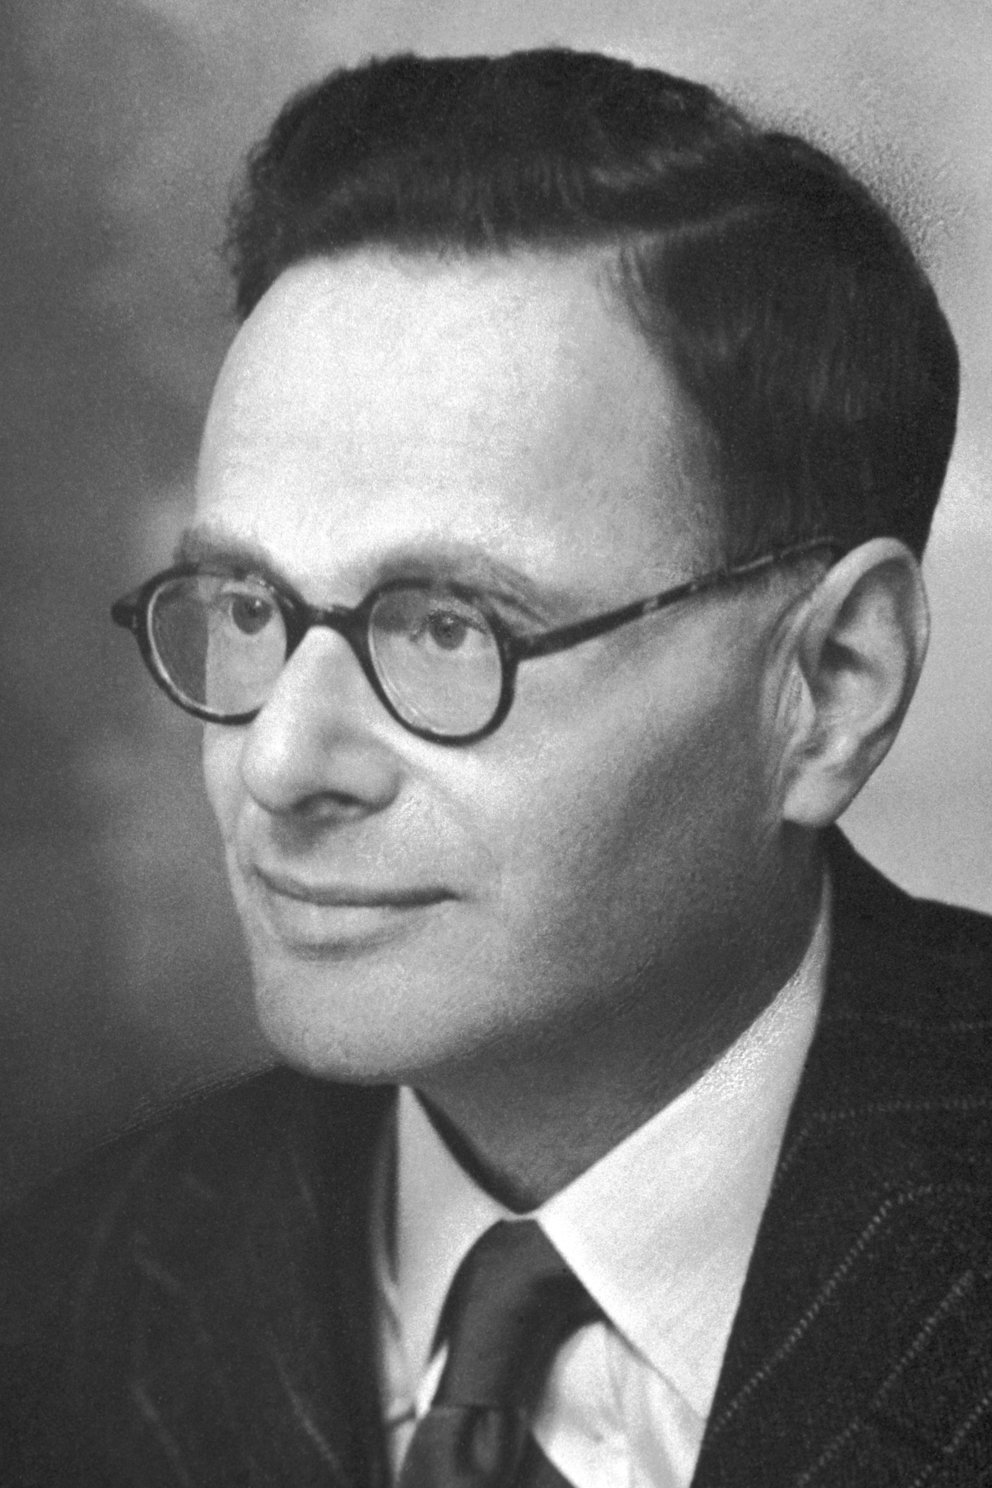
\includegraphics[width=0.26\linewidth]{images/book3/krebs.jpg}

{\small 汉斯·克雷布斯（1900--1981），他于 1937 年根据
绞碎鸽肌氧化其各种酸的速率推出该循环。照片：
诺贝尔基金会，公有领域。}
\end{omfigure}

\section{氧化磷酸化}

\begin{definition}[呼吸链]\label{def:b1:respiration-fermentation:chain}
\index{呼吸链}\index{电子传递链}
\emph{呼吸链}由位于\omterm{def:b1:eukaryotic-cell:mitochondrion}{线粒体}内膜上的四个\omterm{def:b1:proteins:peptide}{蛋白质}复合体和
两种可移动载体构成。NADH 将其电子
交给\emph{复合体 I}，$\mathrm{FADH_2}$（经琥珀酸脱氢酶，
即\emph{复合体 II}）交出自身电子；二者都还原
\emph{泛醌}（Q），一种在膜中扩散的脂溶性醌；
Q 将其传给\emph{复合体 III}，后者再交给
\emph{\omterm{def:b1:cell-unit-of-life:cell}{细胞}色素 $c$}，外侧面上的一种小\omterm{def:b1:proteins:peptide}{蛋白质}；而
\emph{复合体 IV}（\omterm{def:b1:cell-unit-of-life:cell}{细胞}色素氧化酶）每次四个一组地将电子
交给 $\mathrm{O_2}$，生成水。在复合体 I、III 和 IV 处，
电子的电势下降，释放的能量将质子由基质泵入
膜间隙：每对电子分别约为 4、4、2 个质子，
即每个 NADH 为 10 个，每个 $\mathrm{FADH_2}$ 为 6 个（它在
复合体 I 之后进入）。
\end{definition}

\begin{omfigure}
\begin{tikzpicture}[font=\footnotesize, >=Stealth, line cap=round]
  % membrane band
  \fill[omDef!15] (0,0) rectangle (13.0,1.4);
  \draw[omDef!60!black] (0,0) -- (13.0,0) (0,1.4) -- (13.0,1.4);
  \node[anchor=east, gray, align=right] at (-0.15,1.25) {膜间隙 \\ （高 $\mathrm{H^+}$，pH 7）};
  \node[anchor=east, gray, align=right] at (-0.15,0.15) {基质 \\ （低 $\mathrm{H^+}$，pH 8）};
  % complexes
  \node[draw, thick, fill=omThm!25, rounded corners=3pt, minimum height=18mm, minimum width=13mm, align=center] (c1) at (1.5,0.7) {I};
  \node[draw, thick, fill=omThm!25, rounded corners=3pt, minimum height=12mm, minimum width=10mm, align=center] (c2) at (3.6,0.5) {II};
  \node[draw, thick, fill=omThm!25, rounded corners=3pt, minimum height=18mm, minimum width=13mm, align=center] (c3) at (6.2,0.7) {III};
  \node[draw, thick, fill=omThm!25, rounded corners=3pt, minimum height=18mm, minimum width=13mm, align=center] (c4) at (8.9,0.7) {IV};
  \node[draw, thick, fill=omExo!25, rounded corners=6pt, minimum height=16mm, minimum width=12mm, align=center] (atp) at (11.6,0.5) {ATP\\ 合酶};
  \node[circle, draw, thick, fill=omProp!30, inner sep=1.5pt, font=\scriptsize] (q) at (4.9,0.55) {Q};
  \node[circle, draw, thick, fill=omProp!30, inner sep=1.5pt, font=\scriptsize] (cyt) at (7.55,1.25) {细胞色素 $c$};
  % electron flow
  \draw[->, thick, omProp] (c1) -- (q); \draw[->, thick, omProp] (c2) -- (q); \draw[->, thick, omProp] (q) -- (c3); \draw[->, thick, omProp] (c3) -- (cyt); \draw[->, thick, omProp] (cyt) -- (c4);
  % inputs
  \node[anchor=north, align=center] at (1.5,-0.5) {NADH $\to$ $\mathrm{NAD^+}$};
  \node[anchor=north, align=center] at (3.6,-0.5) {$\mathrm{FADH_2}$\\ （琥珀酸）};
  \node[anchor=north, align=center, font=\scriptsize] at (8.6,-0.5) {$\tfrac12\,\mathrm{O_2} + 2\,\mathrm{H^+} \to \mathrm{H_2O}$};
  % proton pumping arrows
  \foreach \x/\n in {1.5/4 $\mathrm{H^+}$, 6.2/4 $\mathrm{H^+}$, 8.9/2 $\mathrm{H^+}$} {
    \draw[->, very thick, omExo!80!black] (\x+0.5,-0.05) -- (\x+0.5,1.9) node[above, font=\scriptsize] {\n};
  }
  \draw[->, very thick, omExo!80!black] (11.6,2.1) -- (11.6,1.35);
  \draw[->, very thick, omExo!80!black] (11.6,-0.35) -- (11.6,-0.75);
  \node[anchor=south, font=\scriptsize] at (11.6,2.15) {每个 ATP 约 $\approx 4\,\mathrm{H^+}$};
  \node[anchor=north, align=center, font=\scriptsize] at (11.6,-0.8) {ADP $+ \mathrm{P_i} \to$ ATP};
\end{tikzpicture}

{\small \omterm{def:b1:eukaryotic-cell:mitochondrion}{线粒体}内膜。电子（橙色）从
NADH 或 $\mathrm{FADH_2}$ 出发，经各复合体传递至氧；
复合体 I、III 和 IV 将质子泵向外侧（绿色）；\omterm{def:b1:water-small-molecules:atp}{ATP} 合酶
使质子回流并合成 \omterm{def:b1:water-small-molecules:atp}{ATP}。}
\end{omfigure}

\begin{theorem}[化学渗透偶联]\label{thm:b1:respiration-fermentation:chemiosmosis}
\index{化学渗透学说}\index{质子动力势}
由\omterm{def:b1:respiration-fermentation:chain}{电子传递链}建立的质子梯度——约 \qty{0.16}{V} 的\omterm{def:b1:membranes-transport:potential}{膜电位}（基质为负）
加上一个 \omterm{def:b1:water-small-molecules:ph}{pH} 单位，即约 \qty{0.22}{V} 的
\emph{质子动力势}，或每摩尔质子 \qty{21}{kJ}——
是电子传递与 \omterm{def:b1:water-small-molecules:atp}{ATP} 合成之间唯一的环节。\omterm{def:b1:water-small-molecules:atp}{ATP} 合酶是内膜上的
一台旋转马达，每合成一个 \omterm{def:b1:water-small-molecules:atp}{ATP} 让约 \qty{3}{H^+} 通过，
另有一个质子用于输入磷酸、输出 \omterm{def:b1:water-small-molecules:atp}{ATP}：每个 \omterm{def:b1:water-small-molecules:atp}{ATP} 共 4 个。
由此得到\emph{P/O 比}\index{P/O 比}：$10/4 = 2.5$，
即每个 NADH 产生 2.5 个 \omterm{def:b1:water-small-molecules:atp}{ATP}；$6/4 = 1.5$，
即每个 $\mathrm{FADH_2}$ 产生 1.5 个 \omterm{def:b1:water-small-molecules:atp}{ATP}。
\end{theorem}
\begin{proof}[证据]
只有内膜完整且封闭的\omterm{def:b1:eukaryotic-cell:mitochondrion}{线粒体}才能合成 \omterm{def:b1:water-small-molecules:atp}{ATP}；
能传递电子却无法维持梯度的碎片则不合成 \omterm{def:b1:water-small-molecules:atp}{ATP}。
解偶联剂（如二硝基苯酚）可穿过膜来回转运质子，
使 \omterm{def:b1:water-small-molecules:atp}{ATP} 合成停止，而耗氧仍然持续，甚至加快，
能量以热的形式散失——棕色\omterm{def:b1:lipids:triglyceride}{脂肪}正是借助自身的
解偶联蛋白有意地这样做（见\cref{ch:b1:mammal-organization}）。
二硝基苯酚曾被当作减肥药出售，却因体温过高而致人死亡。
\omterm{def:b1:respiration-fermentation:chain}{电子传递链}的\omterm{def:b1:enzymes:inhibitors}{抑制剂}（如作用于复合体 IV 的氰化物）同时阻断两者；
\omterm{def:b1:water-small-molecules:atp}{ATP} 合酶的\omterm{def:b1:enzymes:inhibitors}{抑制剂}（寡霉素）阻断 \omterm{def:b1:water-small-molecules:atp}{ATP} 合成，
由于梯度无法释放，呼吸也随之停止，
此时加入解偶联剂又可使呼吸恢复。在黑暗中人为施加于\omterm{def:b1:eukaryotic-cell:mitochondrion}{线粒体}的 \omterm{def:b1:water-small-molecules:ph}{pH} 梯度
可驱动 \omterm{def:b1:water-small-molecules:atp}{ATP} 合成，与\omterm{def:b1:photosynthesis:chloroplast}{叶绿体}中的情形相同
（见\cref{ch:b1:photosynthesis}）。
\end{proof}

\begin{omfigure}
\begin{tikzpicture}
  \node[anchor=south west, inner sep=0] (img) at (0,0)
    {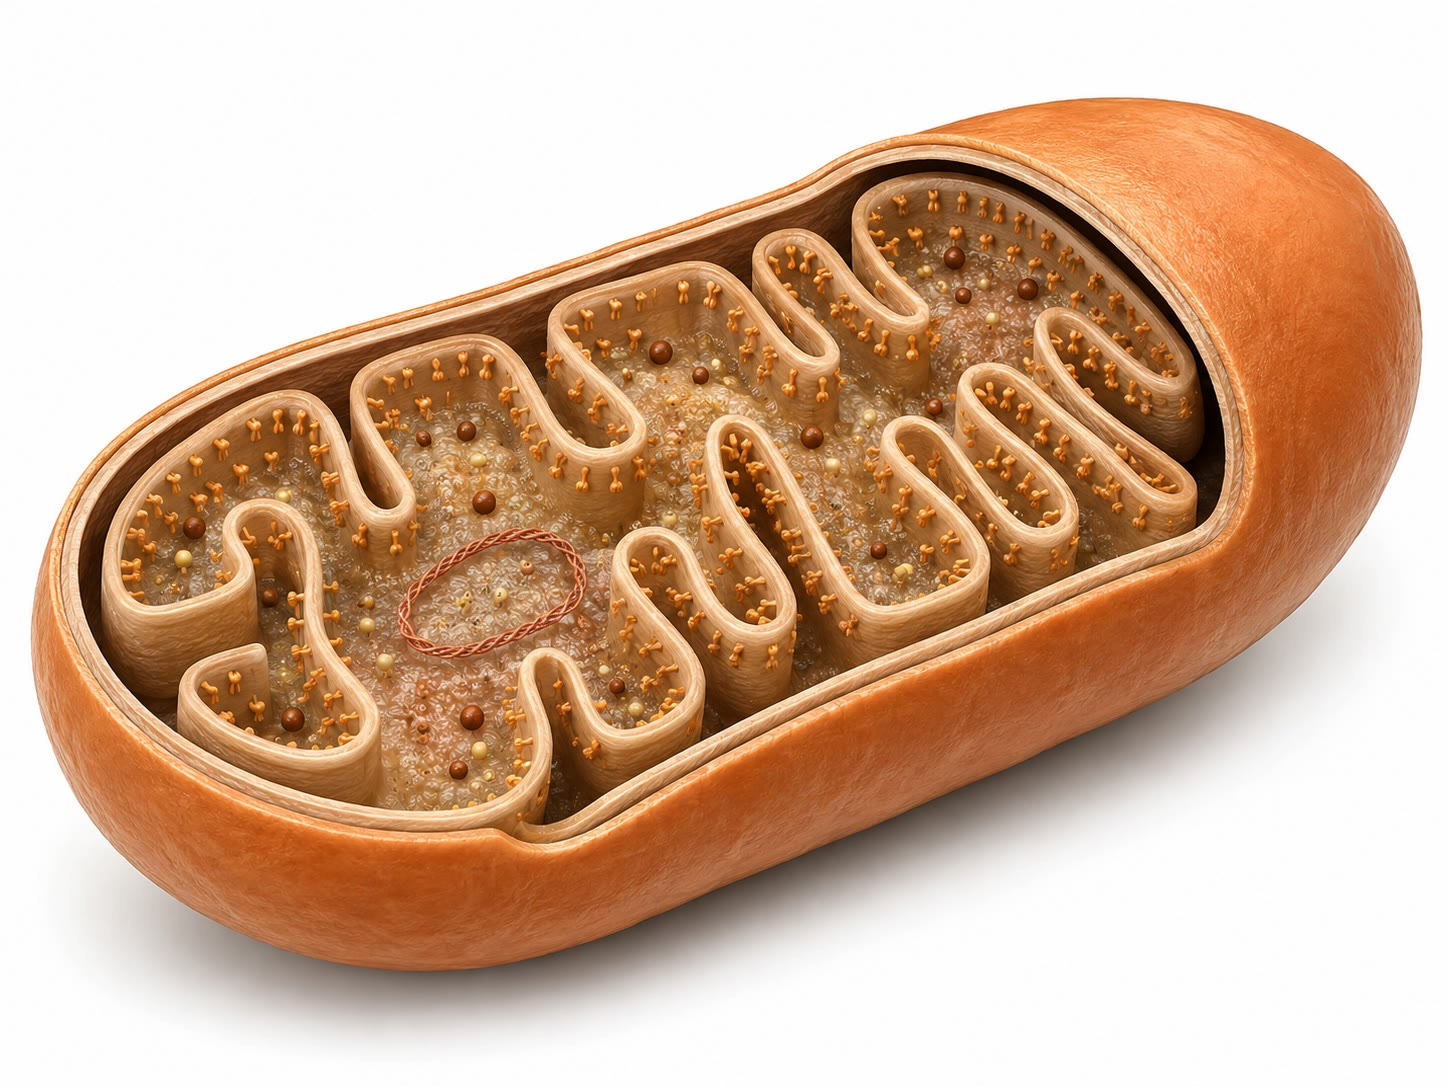
\includegraphics[width=0.54\linewidth]{images/book3/ai/fig-mitochondrion-cutaway.jpg}};
  \begin{scope}[x={(img.south east)}, y={(img.north west)},
      every node/.style={font=\small}]
    \draw[omDef, thick] (0.10,0.55) -- (-0.03,0.70) node[left] {外膜};
    \draw[omDef, thick] (0.45,0.72) -- (0.45,1.08) node[above, align=center] {内膜折叠形成嵴：\\ 呼吸链与 ATP 合酶};
    \draw[omDef, thick] (0.55,0.35) -- (1.03,0.24) node[right, align=left] {基质：克雷布斯循环，\\ DNA、核糖体};
    \draw[omDef, thick] (0.16,0.40) -- (-0.03,0.26) node[left] {膜间隙};
  \end{scope}
\end{tikzpicture}

{\small 剖开的\omterm{def:b1:eukaryotic-cell:mitochondrion}{线粒体}示意图。内膜的折叠增加了
\omterm{def:b1:respiration-fermentation:chain}{呼吸链}与 \omterm{def:b1:water-small-molecules:atp}{ATP} 合酶可利用的面积；其内的基质
容纳\omterm{def:b1:respiration-fermentation:krebs}{克雷布斯循环}。}
\end{omfigure}

\begin{method}[一个葡萄糖的 ATP 收支]\label{met:b1:respiration-fermentation:balance}
\begin{enumerate}
  \item \omterm{def:b1:respiration-fermentation:glycolysis}{糖酵解}：净得 $+2$ 个 \omterm{def:b1:water-small-molecules:atp}{ATP}，并在\omterm{def:b1:eukaryotic-cell:organelle}{细胞溶胶}中产生 $+2$ 个 NADH。
  \item 丙酮酸脱氢酶：$+2$ 个 NADH。\omterm{def:b1:respiration-fermentation:krebs}{克雷布斯循环}：$+6$ 个 NADH，$+2$
        个 $\mathrm{FADH_2}$，$+2$ 个 GTP（$=$ \omterm{def:b1:water-small-molecules:atp}{ATP}）。
  \item 氧化磷酸化：每个\omterm{def:b1:eukaryotic-cell:mitochondrion}{线粒体} NADH 产生 $2.5$ 个 \omterm{def:b1:water-small-molecules:atp}{ATP}
        （8 个：20 个 \omterm{def:b1:water-small-molecules:atp}{ATP}），$1.5$ 个 \omterm{def:b1:water-small-molecules:atp}{ATP} 来自每个 $\mathrm{FADH_2}$（2 个：3 个 \omterm{def:b1:water-small-molecules:atp}{ATP}）。
  \item \omterm{def:b1:eukaryotic-cell:organelle}{细胞溶胶}中的 NADH 不能穿过内膜，其电子
        须经穿梭机制进入\omterm{def:b1:eukaryotic-cell:mitochondrion}{线粒体}，该机制将电子交给 $\mathrm{FAD}$
        （肌肉和脑中每个 1.5 个 \omterm{def:b1:water-small-molecules:atp}{ATP}），或交给 $\mathrm{NAD^+}$（肝脏和心脏中每个 2.5
        个 \omterm{def:b1:water-small-molecules:atp}{ATP}），即 3 个或 5 个 \omterm{def:b1:water-small-molecules:atp}{ATP}。
  \item 合计：$2 + 2 + 20 + 3 + 3 = 30$，
        若用较好的穿梭机制则为 $32$。在\omterm{def:b1:cell-unit-of-life:cell}{细胞}条件下，效率为
        $30\times 50/2870 \approx \qty{52}{\%}$。
\end{enumerate}
\end{method}

\section{发酵}

\begin{definition}[发酵]\label{def:b1:respiration-fermentation:fermentation}
\index{发酵}
没有氧气时，\omterm{def:b1:respiration-fermentation:chain}{呼吸链}停止工作，NADH 无法被再氧化，
\omterm{def:b1:respiration-fermentation:glycolysis}{糖酵解}会因缺少 $\mathrm{NAD^+}$ 而在几秒内停止。
\emph{发酵}使其得以再生，其方式是以丙酮酸本身作
为电子受体：在\emph{乳酸发酵}（肌肉、红\omterm{def:b1:cell-unit-of-life:cell}{细胞}、乳酸菌）中，
丙酮酸被还原为乳酸；在\emph{酒精发酵}（酵母、某些植物）中，
丙酮酸脱羧生成乙醛，
乙醛再被还原为乙醇，并释放 $\mathrm{CO_2}$。发酵的产量
仅来自\omterm{def:b1:respiration-fermentation:glycolysis}{糖酵解}本身：每个葡萄糖得 2 个 \omterm{def:b1:water-small-molecules:atp}{ATP}，
仅为呼吸作用的十五分之一；碳几乎没有被氧化，
产物中仍保留着燃料几乎全部的能量。\emph{无氧呼吸}——
以硝酸盐、硫酸盐或碳酸盐代替氧作为末端电子受体的\omterm{def:b1:respiration-fermentation:chain}{电子传递链}，
存在于许多细菌中——是另一回事，将在本科二年级分册中讨论。
\end{definition}

\begin{omfigure}
\begin{minipage}[b]{0.44\linewidth}\centering
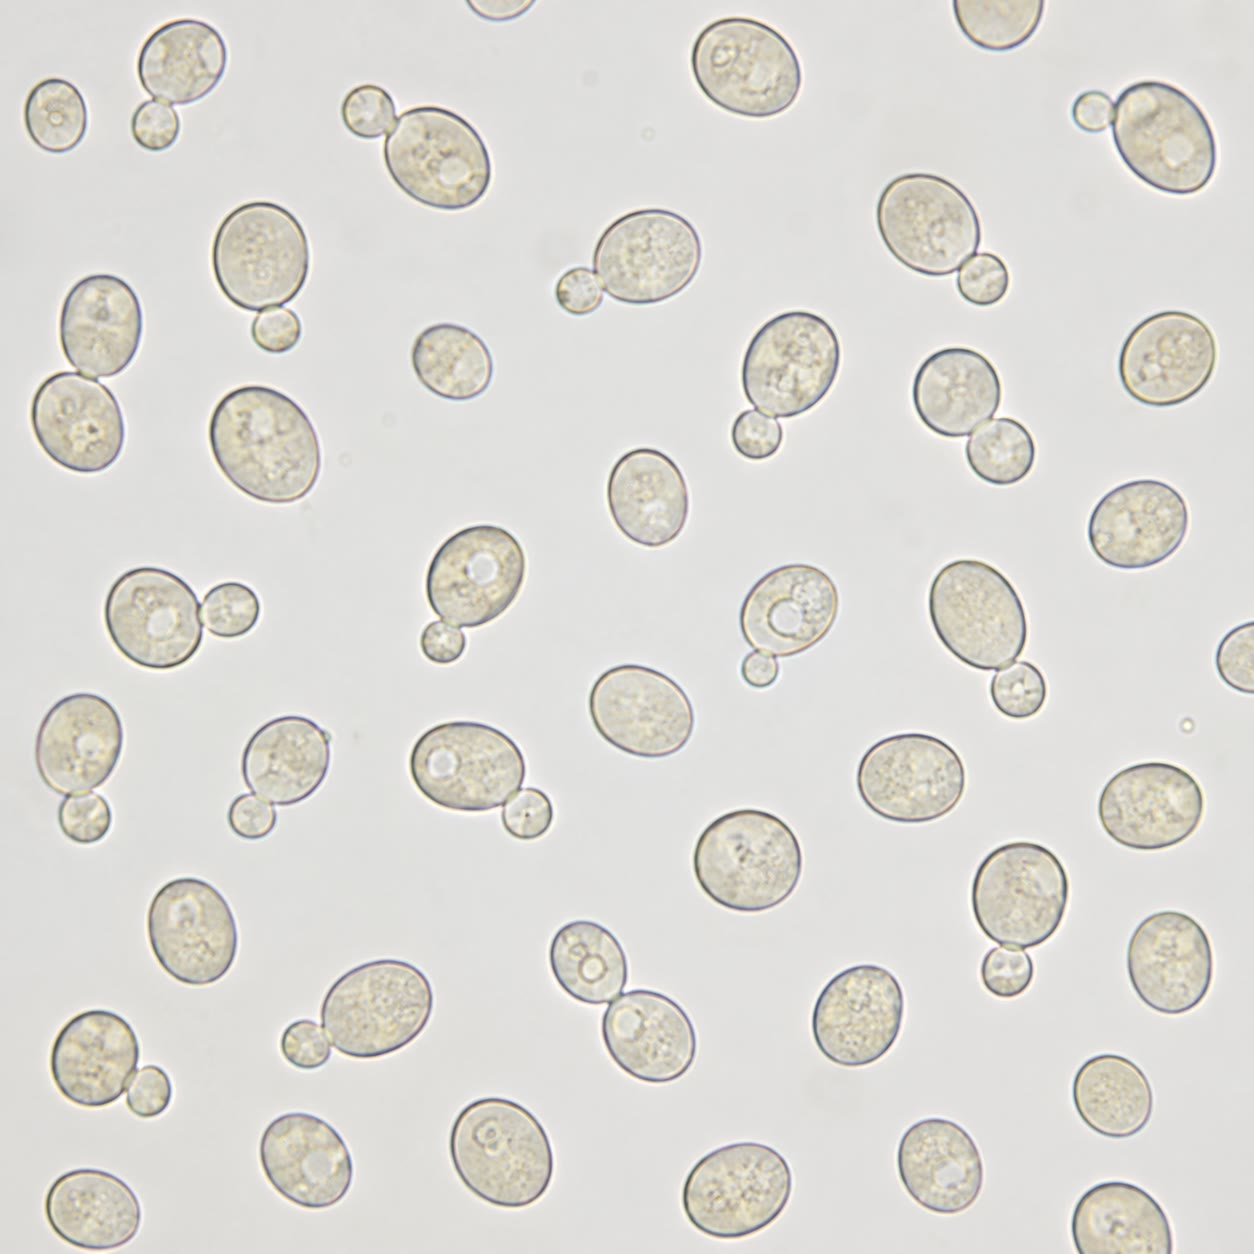
\includegraphics[width=0.9\linewidth]{images/book3/ai/b3-15-yeast-budding.jpg}
\end{minipage}\hfill
\begin{minipage}[b]{0.52\linewidth}\centering
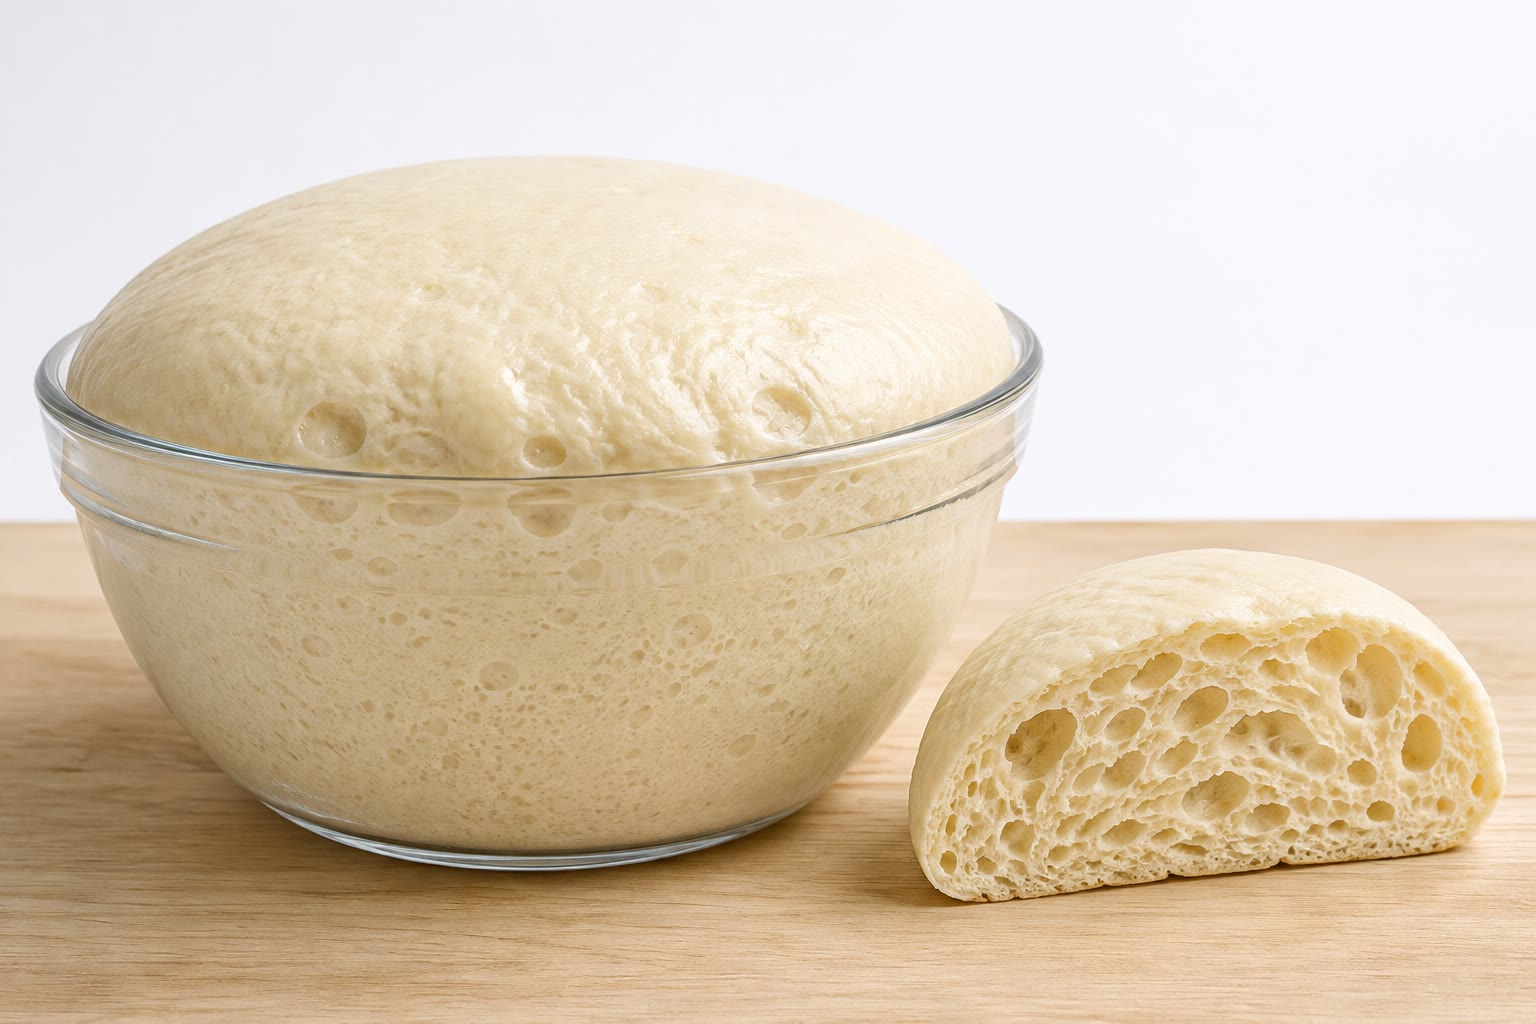
\includegraphics[width=0.96\linewidth]{images/book3/ai/b3-15-bread-dough-risen.jpg}
\end{minipage}

{\small 左：面包酵母，正在出芽。右：其\omterm{def:b1:respiration-fermentation:fermentation}{发酵}对面团的作用：
每个葡萄糖经\omterm{def:b1:respiration-fermentation:glycolysis}{糖酵解}得两个 \omterm{def:b1:water-small-molecules:atp}{ATP} 所对应的 $\mathrm{CO_2}$，
被截留在面筋之中。乙醇在烘烤中挥发。}
\end{omfigure}

\begin{proposition}[巴斯德效应]\label{prop:b1:respiration-fermentation:pasteur}
\index{巴斯德效应}
能够进行呼吸作用的\omterm{def:b1:cell-unit-of-life:cell}{细胞}，缺氧时消耗葡萄糖的速度远快于供氧时，
而其生长远为缓慢。
\end{proposition}
\begin{proof}[证据]
巴斯德（1861 年）发现，在通气的\omterm{def:b1:respiration-fermentation:fermentation}{发酵}罐中，酵母消耗糖分缓慢，
并不断繁殖；而在密闭的\omterm{def:b1:respiration-fermentation:fermentation}{发酵}罐中，其消耗糖分的速度快了十倍，
繁殖甚少，并生成了酒精。其解释在于 \omterm{def:b1:water-small-molecules:atp}{ATP}
产量：若每个葡萄糖只产生 2 个 \omterm{def:b1:water-small-molecules:atp}{ATP}，要获得与 30 个 \omterm{def:b1:water-small-molecules:atp}{ATP} 相同的量，\omterm{def:b1:cell-unit-of-life:cell}{细胞}
必须使\omterm{def:b1:respiration-fermentation:glycolysis}{糖酵解}快十五倍，而呼吸作用所维持的
\omterm{def:b1:water-small-molecules:atp}{ATP} 与柠檬酸对 PFK 的抑制被解除，使\omterm{def:b1:cell-unit-of-life:cell}{细胞}得以如此。
短跑中的肌肉在数秒内即呈现同样的效应：其\omterm{def:b1:carbohydrates:polysaccharide}{糖原}
消耗速度为静息时的二十倍，同时乳酸上升。
\end{proof}

\begin{definition}[呼吸商]\label{def:b1:respiration-fermentation:rq}
\index{呼吸商}
\emph{呼吸商}RQ 是所产生的 $\mathrm{CO_2}$ 与所消耗的
$\mathrm{O_2}$ 之比，以摩尔计。碳水化合物为 1.0
（每个葡萄糖分子中两者各为六个）；\omterm{def:b1:lipids:triglyceride}{脂肪}约为 0.7（以棕榈酸为例：
$\mathrm{C_{16}H_{32}O_2} + 23\,\mathrm{O_2} \to 16\,\mathrm{CO_2} +
16\,\mathrm{H_2O}$，$16/23 = 0.70$），因其碳原子还原程度更高，
每释放一个 $\mathrm{CO_2}$ 所需的氧更多；\omterm{def:b1:proteins:peptide}{蛋白质}约为 0.8。
\omterm{def:b1:respiration-fermentation:fermentation}{发酵}培养物在不吸入氧的情况下释放 $\mathrm{CO_2}$：其
RQ 为无穷大，而混合培养物的 RQ 若超过 1，则表明其中
\omterm{def:b1:respiration-fermentation:fermentation}{发酵}所占的比例。若以气体分析测量整个动物，RQ 可说明
它在燃烧何种燃料。
\end{definition}

\begin{example}[读取 RQ]\label{ex:b1:respiration-fermentation:readrq}
静息状态的人进食碳水化合物餐后：RQ 为 0.95，正在燃烧葡萄糖。
同一人禁食一夜后：RQ 为 0.75，燃烧\omterm{def:b1:lipids:triglyceride}{脂肪}。一名马拉松选手在
第三十公里处，\omterm{def:b1:carbohydrates:polysaccharide}{糖原}已耗尽：RQ 为 0.72。一瓶酵母
在葡萄糖中并通入少量空气：RQ 为 4——其葡萄糖的四分之三
正在被\omterm{def:b1:respiration-fermentation:fermentation}{发酵}。
\end{example}

\section{其他燃料与整体的调节}

\begin{proposition}[脂肪和蛋白质进入同一套代谢机制]\label{prop:b1:respiration-fermentation:otherfuels}
\index{$\beta$-氧化}
\omterm{def:b1:lipids:fattyacid}{脂肪酸}先活化为酰基\omterm{def:b1:enzymes:enzyme}{辅酶} A，并在\omterm{def:b1:eukaryotic-cell:mitochondrion}{线粒体}
基质中经 \emph{$\beta$-氧化}每次缩短两个碳原子，
每一轮产生一个乙酰\omterm{def:b1:enzymes:enzyme}{辅酶} A、一个 NADH 和一个 $\mathrm{FADH_2}$：
棕榈酸（C16）可得 8 个乙酰\omterm{def:b1:enzymes:enzyme}{辅酶} A、7 个 NADH 和 7 个 $\mathrm{FADH_2}$——
约 106 个 \omterm{def:b1:water-small-molecules:atp}{ATP}，即每个碳原子约 \qty{6.6}{} 个 \omterm{def:b1:water-small-molecules:atp}{ATP}，葡萄糖则为 5 个。
\omterm{def:b1:proteins:aminoacid}{氨基酸}以氨的形式失去氮（氨在
肝脏中转化为尿素），其碳骨架以丙酮酸、乙酰\omterm{def:b1:enzymes:enzyme}{辅酶} A 或
\omterm{def:b1:respiration-fermentation:krebs}{克雷布斯循环}中间体的形式进入代谢。所有燃料汇聚于乙酰\omterm{def:b1:enzymes:enzyme}{辅酶} A 与
\omterm{def:b1:respiration-fermentation:chain}{呼吸链}；\omterm{def:b1:cell-unit-of-life:cell}{细胞}依据激素以及自身 \omterm{def:b1:water-small-molecules:atp}{ATP} 的状态在其间作出选择，
如\cref{ch:b1:biosyntheses-integration}所述。
\end{proposition}

\begin{example}[各一克的对比]\label{ex:b1:respiration-fermentation:gramofeach}
一克葡萄糖（\qty{5.6}{mmol}）可产生约 \qty{170}{mmol} 的
\omterm{def:b1:water-small-molecules:atp}{ATP}；一克棕榈酸（\qty{3.9}{mmol}）约产生 \qty{410}{mmol}——
\qty{38}{kJ/g}，对比 \cref{ch:b1:lipids}中的 \qty{17}{kJ/g}，
换算成了通用的能量货币。\omterm{def:b1:lipids:triglyceride}{脂肪}每生成一个 \omterm{def:b1:water-small-molecules:atp}{ATP} 需要的氧更多，这正是
为何缺氧的冲刺肌肉燃烧\omterm{def:b1:carbohydrates:polysaccharide}{糖原}，而迁徙的鸟
类氧气充足而质量受限，燃烧\omterm{def:b1:lipids:triglyceride}{脂肪}。
\end{example}

\section{练习}

\begin{exercise}[$\star$]\label{exo:b1:respiration-fermentation:1}
说出呼吸作用的三个阶段、它们所在的位置，以及各阶段
分别产生什么。
\end{exercise}

\begin{exercise}[$\star$]\label{exo:b1:respiration-fermentation:2}
写出\omterm{def:b1:respiration-fermentation:glycolysis}{糖酵解}的总平衡式，并说明“\omterm{def:b1:respiration-fermentation:glycolysis}{底物水平
磷酸化}”。
\end{exercise}

\begin{exercise}[$\star$]\label{exo:b1:respiration-fermentation:3}
根据\omterm{def:b1:respiration-fermentation:krebs}{克雷布斯循环}图，依次列出一轮循环中释放的产物，
并说明两个 $\mathrm{CO_2}$ 各来自何处。
\end{exercise}

\begin{exercise}[$\star$]\label{exo:b1:respiration-fermentation:4}
在无氧条件下，\omterm{def:b1:respiration-fermentation:fermentation}{发酵}为\omterm{def:b1:cell-unit-of-life:cell}{细胞}完成了什么，
又未能完成什么？
\end{exercise}

\begin{exercise}[$\star\star$]\label{exo:b1:respiration-fermentation:5}
计算两个电子从 NADH 转移时的 $\Delta G^{\circ\prime}$：
NADH（$E'_0 = \qty{-0.32}{V}$）传给氧（\qty{+0.82}{V}）以及
传给泛醌（\qty{+0.05}{V}）时的该值。每一步原则上
可支付多少个 \omterm{def:b1:water-small-molecules:atp}{ATP}？
\end{exercise}

\begin{exercise}[$\star\star$]\label{exo:b1:respiration-fermentation:6}
列出一个葡萄糖在肌肉\omterm{def:b1:cell-unit-of-life:cell}{细胞}（甘油-3-磷酸穿梭）中的 \omterm{def:b1:water-small-molecules:atp}{ATP} 收支，
以及在肝\omterm{def:b1:cell-unit-of-life:cell}{细胞}（苹果酸穿梭）中的 \omterm{def:b1:water-small-molecules:atp}{ATP} 收支，并取 \omterm{thm:b1:respiration-fermentation:chemiosmosis}{P/O
比}分别为 2.5 和 1.5。
\end{exercise}

\begin{exercise}[$\star\star$]\label{exo:b1:respiration-fermentation:7}
某培养物以葡萄糖为\omterm{def:b1:enzymes:enzyme}{底物}，每小时消耗 \qty{1.0}{mmol} 的 $\mathrm{O_2}$，
并释放 \qty{2.2}{mmol} 的 $\mathrm{CO_2}$。计算
RQ，以及被呼吸与被\omterm{def:b1:respiration-fermentation:fermentation}{发酵}的葡萄糖各占的比例。
\end{exercise}

\begin{exercise}[$\star\star$]\label{exo:b1:respiration-fermentation:8}
解释向进行呼吸的\omterm{def:b1:eukaryotic-cell:mitochondrion}{线粒体}中加入二硝基苯酚后，耗氧量、
\omterm{def:b1:water-small-molecules:atp}{ATP} 合成和产热各会发生什么变化，
以及这种药物为何会致死。
\end{exercise}

\begin{exercise}[$\star\star$]\label{exo:b1:respiration-fermentation:9}
氰化物会抑制复合体 IV。预测其对\omterm{def:b1:cell-unit-of-life:cell}{细胞}中\omterm{def:b1:respiration-fermentation:chain}{呼吸链}的影响，
对\omterm{def:b1:respiration-fermentation:krebs}{克雷布斯循环}和\omterm{def:b1:respiration-fermentation:glycolysis}{糖酵解}的影响，
并解释中毒者血液中为何会积累乳酸。
\end{exercise}

\begin{exercise}[$\star\star\star$]\label{exo:b1:respiration-fermentation:10}
计算棕榈酸的 \omterm{def:b1:water-small-molecules:atp}{ATP} 产量（8 个乙酰\omterm{def:b1:enzymes:enzyme}{辅酶} A、7 个 NADH、7 个
$\mathrm{FADH_2}$，减去活化所消耗的 2 个 \omterm{def:b1:water-small-molecules:atp}{ATP}），并计算其每个碳原子的 \omterm{def:b1:water-small-molecules:atp}{ATP} 产量；
分别计算棕榈酸和葡萄糖每产生一个 \omterm{def:b1:water-small-molecules:atp}{ATP} 所消耗的氧气量；
潜水海豹和蜂鸟各应优先利用哪种燃料？
\end{exercise}

\begin{exercise}[$\star\star\star$]\label{exo:b1:respiration-fermentation:11}
一根肌纤维中含有 \qty{5}{mmol/L} 的 \omterm{def:b1:water-small-molecules:atp}{ATP}，在短跑中以 \qty{3}{mmol/L}
每秒的速率消耗。仅依靠这些 \omterm{def:b1:water-small-molecules:atp}{ATP}，它能维持多久？其磷酸肌酸
（\qty{25}{mmol/L}）可一对一地再生 \omterm{def:b1:water-small-molecules:atp}{ATP}；
其\omterm{def:b1:carbohydrates:polysaccharide}{糖原}经\omterm{def:b1:respiration-fermentation:fermentation}{发酵}，每个葡萄糖单位产生 3 个 \omterm{def:b1:water-small-molecules:atp}{ATP}，速率最高可达
\qty{2}{mmol/L} 葡萄糖单位每秒。计算每种储备
能维持这段短跑的时间，并解释为何 100 m 赛跑
几乎完全在无氧条件下进行。
\end{exercise}

\begin{exercise}[$\star\star\star$]\label{exo:b1:respiration-fermentation:12}
“\omterm{def:b1:eukaryotic-cell:mitochondrion}{线粒体}是一块由电子充电、经由
涡轮机放电的电池。”用一段文字讨论：梯度储存了什么，
合酶做了什么，这一类比在哪些方面是精确的，在哪些方面
是粗略的。
\end{exercise}

\section{问题：有氧与无氧条件下的酵母}

\begin{problem}[{周末问题——重温巴斯德的发酵罐：计数 ATP、测定葡萄糖消耗、
生物量增长与气体测定，最后归结为 ATP 产量之比与 P/O
比}]
\label{pb:b1:respiration-fermentation:1}
酵母以葡萄糖为\omterm{def:b1:enzymes:enzyme}{底物}，在两个相同的烧瓶中培养，一个通气，一个密封。
取 P/O 比：NADH 为 2.5，$\mathrm{FADH_2}$ 为 1.5，
以 $\mathrm{FADH_2}$ 穿梭途径处理胞质 NADH，生长产率为
每摩尔 \omterm{def:b1:water-small-molecules:atp}{ATP} 产生 \qty{10.5}{g} 干生物量，葡萄糖的摩尔质量取
\qty{180}{g/mol}。

\medskip
\noindent\textbf{第一部分——计数 \omterm{def:b1:water-small-molecules:atp}{ATP}。}
\begin{enumerate}
  \item 列出一个葡萄糖经\omterm{def:b1:respiration-fermentation:glycolysis}{糖酵解}、丙酮酸脱氢酶反应和
        \omterm{def:b1:respiration-fermentation:krebs}{克雷布斯循环}产生的
        \omterm{def:b1:water-small-molecules:atp}{ATP}、GTP、NADH 和 $\mathrm{FADH_2}$。
  \item 计算每个葡萄糖经\omterm{def:b1:respiration-fermentation:chain}{呼吸链}泵出的质子数
        （\omterm{def:b1:eukaryotic-cell:mitochondrion}{线粒体} NADH 每个 10 个，$\mathrm{FADH_2}$ 每个 6 个；胞质 NADH
        以 $\mathrm{FADH_2}$ 形式进入）。
  \item 以每产生一个 \omterm{def:b1:water-small-molecules:atp}{ATP} 需 \qty{4}{H^+} 计，计算合酶产生的 \omterm{def:b1:water-small-molecules:atp}{ATP} 数，
        并求有氧条件下每个葡萄糖的总 \omterm{def:b1:water-small-molecules:atp}{ATP} 产量。
  \item 求无氧条件下每个葡萄糖的 \omterm{def:b1:water-small-molecules:atp}{ATP} 产量。
  \item 求两者产量之比。
  \item 求有氧条件下捕获的\omterm{prop:b1:water-small-molecules:gibbs}{自由能}（$\Delta G_{\text{ATP}}
        = \qty{-50}{kJ/mol}$）占 \qty{2870}{kJ} 的比例，并求
        无氧条件下占 \qty{2870}{kJ} 的比例，以及
        占\omterm{def:b1:respiration-fermentation:fermentation}{发酵}实际释放能量（葡萄糖生成两个
        乙醇和两个 $\mathrm{CO_2}$：\qty{-235}{kJ/mol}）的比例。
\end{enumerate}

\medskip
\noindent\textbf{第二部分——葡萄糖消耗与生物量增长。}
密封烧瓶为维持其\omterm{def:b1:cell-unit-of-life:cell}{细胞}，必须以与通气烧瓶相同的速率产生 \omterm{def:b1:water-small-molecules:atp}{ATP}，
即每小时 \qty{30}{mmol} \omterm{def:b1:water-small-molecules:atp}{ATP}。
\begin{enumerate}[resume]
  \item 求每个烧瓶每小时消耗的葡萄糖量。
  \item 求密封烧瓶每小时产生的乙醇和 $\mathrm{CO_2}$，
        以及通气烧瓶中交换的 $\mathrm{CO_2}$ 和
        $\mathrm{O_2}$ 的量。
  \item 求密封烧瓶每摩尔葡萄糖所能合成的生物量，
        以及每克葡萄糖所能合成的生物量。
  \item 通气烧瓶每克葡萄糖合成 \qty{0.5}{g} 生物量。以
        \qty{10.5}{g/mol} 计，求这相当于多少 \omterm{def:b1:water-small-molecules:atp}{ATP}，
        并与可用的 30 个 \omterm{def:b1:water-small-molecules:atp}{ATP} 比较。是什么
        限制了有氧条件下的产率？
  \item 结合第 7 题和第 9 题，解释\omterm{prop:b1:respiration-fermentation:pasteur}{巴斯德效应}，
        并指出实现该效应的调控所针对的酶。
\end{enumerate}

\medskip
\noindent\textbf{第三部分——气体测定。}
第三个烧瓶通气不足，每小时释放 \qty{44}{mg} 的 $\mathrm{CO_2}$，
并每小时消耗 \qty{20}{mg} 的 $\mathrm{O_2}$。
\begin{enumerate}[resume]
  \item 将两者换算为毫摩尔，并求 RQ。
  \item 设 $x$ 为每小时被呼吸的葡萄糖量，$y$ 为每小时被\omterm{def:b1:respiration-fermentation:fermentation}{发酵}的葡萄糖量。
        列出 $\mathrm{O_2}$ 和 $\mathrm{CO_2}$ 的物质平衡，
        并解出 $x$ 和 $y$。
  \item 被\omterm{def:b1:respiration-fermentation:fermentation}{发酵}的葡萄糖占多大比例？
        \omterm{def:b1:water-small-molecules:atp}{ATP} 中有多大比例来自\omterm{def:b1:respiration-fermentation:fermentation}{发酵}？
  \item 同一烧瓶改以棕榈酸代替葡萄糖（有氧）：
        求其 RQ。
  \item 某学生测得静息动物在禁食一夜后的 RQ 为 0.7，进食后为 1.0。
        请解释这一结果。
\end{enumerate}

\medskip
\noindent\textbf{第四部分——涡轮机。}
\begin{enumerate}[resume]
  \item 求一摩尔质子穿过质子动力势
        为 \qty{0.22}{V} 时的\omterm{prop:b1:water-small-molecules:gibbs}{自由能}。
  \item 求 \qty{4}{H^+} 的能量，以及合酶的效率，
        取每个 \omterm{def:b1:water-small-molecules:atp}{ATP} 为 \qty{50}{kJ}。
  \item 求两个电子从 NADH 落至 $\mathrm{O_2}$ 时
        释放的\omterm{prop:b1:water-small-molecules:gibbs}{自由能}（\qty{1.14}{V}），
        被泵出的十个质子所储存的能量，以及\omterm{def:b1:respiration-fermentation:chain}{呼吸链}的效率。
  \item 合并两个效率，并与 2.5 个 \omterm{def:b1:water-small-molecules:atp}{ATP} $\times$
        \qty{50}{kJ} 除以 \qty{220}{kJ} 相比较。
  \item 向通气烧瓶中加入解偶联剂，预测其
        耗氧量、\omterm{def:b1:water-small-molecules:atp}{ATP} 产量、葡萄糖消耗、产热
        及生长方面的变化。
  \item 改为加入阻断合酶的寡霉素，
        预测其变化，并说明随后再加入解偶联剂
        会发生什么。
  \item 一株突变酵母缺少复合体 I；其 NADH
        经一种不泵出质子的替代酶进入\omterm{def:b1:respiration-fermentation:chain}{呼吸链}。求
        其 NADH 的 P/O 比和每个葡萄糖的 \omterm{def:b1:water-small-molecules:atp}{ATP} 产量。
  \item 解释无氧时\omterm{def:b1:cell-unit-of-life:cell}{细胞}为何使\omterm{def:b1:eukaryotic-cell:mitochondrion}{线粒体} NADH 池
        几乎保持完全还原，以及这对\omterm{def:b1:respiration-fermentation:krebs}{克雷布斯循环}
        有何影响。
  \item 陈述结果：有氧与无氧条件下每个葡萄糖的 \omterm{def:b1:water-small-molecules:atp}{ATP} 产量、
        二者之比，以及 NADH 和 $\mathrm{FADH_2}$ 的 P/O 比。
\end{enumerate}
\end{problem}
